\chapter{Results}
\label{c:result}

\section{Account registration}


\section{Data source discovery}

% checksum check

\section{Experiment design}

% condition
% simple and advanced mode

\section{RNA-Seq analysis submission}

\section{DNA-Seq anlaysis submission}

\section{Job queue monitoring}

% email notification

\section{Report and result access}

\subsection{Integration with public genome browser}


\section{RNA-Seq analysis result}

\subsection{QC}

\subsection{Alignment - STAR}

\subsection{Alignment - HISAT2}

\subsection{Cufflinks}

\subsection{featureCounts}

\subsection{DESeq2}


\section{DNA-Seq analysis result}

\subsection{QC}

\subsection{Alignment - BWA MEM}

\subsection{Variant calling - Varscan}

\subsection{Variant calling - GATK}

% There is a tree in Figure~%\ref{i:tree}.
% This is English line spacing test. You should see double spacing text.
% This is English line spacing test. You should see double spacing text.
% This is English line spacing test. You should see double spacing text.

%i:tree
%\begin{figure}[!htbp]
\centering
\tikzset{every tree node/.style={align=center},
    level distance=40pt,
    sibling distance=6pt}
\begin{tikzpicture}
\Tree[.root
       [ (a) ]
       [.node
         [.node
           [ (b) ]
           [ (c) ]
         ]
         [.node
           [ (d) ]
           [ (e) ]
           [ (f) ]
           [ (g) ]
           [ (h) ]
         ]
       ]
     ]

\end{tikzpicture}

\caption{A tree. }
\label{i:tree}
\end{figure}


% There is a barchart in Figure~%\ref{i:barchart}.
% This is English line spacing test. You should see double spacing text.
% This is English line spacing test. You should see double spacing text.
% This is English line spacing test. You should see double spacing text.

%i:barchart
%\begin{figure}[!htbp]
    \centering
    \vspace{2em}
    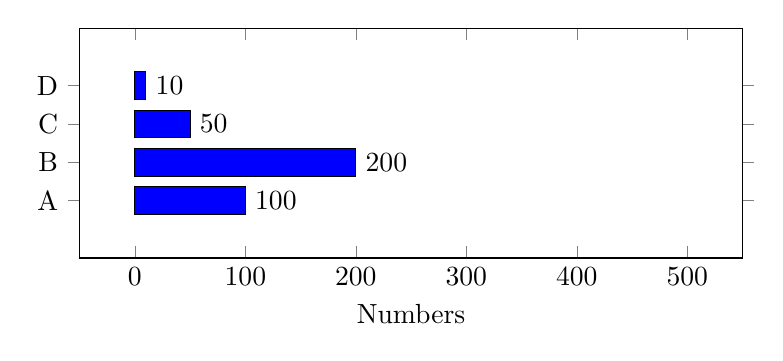
\begin{tikzpicture}
        \begin{axis}[
            enlarge y limits=0.5,
            enlarge x limits=0.1,
            height=4.5cm,
            width=10cm,
            symbolic y coords={A,B,C,D},
            xmin=0,
            xmax=500,
            xbar=1pt,
            xlabel=Numbers,
            nodes near coords={\pgfmathprintnumber[/pgf/number format/assume math mode]{\pgfplotspointmeta}},
            nodes near coords align={horizontal},
            every node near coord/.append style={
                anchor=west}
            ,
            xticklabel style={/pgf/number format/assume math mode},
            yticklabel style={/pgf/number format/assume math mode},
            ytick=data
          ]
            \addplot[xbar,fill=blue] coordinates {
            (100,A)
            (200,B)
            (50,C)
            (10,D)
            };
        \end{axis}
    \end{tikzpicture}
    \caption{A barchart.}
    \label{i:barchart}
\end{figure}


% Our method outperforms state-of-art systems as shown in Table~\ref{t:results}.
% This is English line spacing test. You should see double spacing text.
% This is English line spacing test. You should see double spacing text.
% This is English line spacing test. You should see double spacing text.

%t:results
% \begin{table}[!htbp]
\caption{Final performance of our system. }
\label{t:results} 
\centering
\begin{tabular}{|c|c|c|c|}
\hline

Method      &    Precision &     Recall &     F1-Score \\ \hline
their model &     3.40     &      3.40  &      3.40    \\ \hline
our model   &    99.99     &     99.99  &     99.99    \\ \hline


\end{tabular}
\end{table}

% \begin{table}[!htbp]
\caption[mirDeep2 result summary of both novel and known miRNA.]{mirDeep2 result summary of both novel and known miRNA. Here we can put some very lengthy descriptions as our table legend, and it will not ruin the list of tables, which will only display the shorten version of the caption.}
\label{t:all-sum}
\centering
\begin{threeparttable}
	\begin{tabular}{ccccccc}
	\toprule
    & \multicolumn{3}{c}{novel miRNAs} & \multicolumn{3}{c}{known miRNAs}\\
    \cmidrule(r){2-4} \cmidrule(r){5-7}
    miRDeep2 &       & estimated & estimated  &       &       &  \\
    score & predicted &  false positives\tnote{$\ast$} & true positives\tnote{$\dagger$} & in species & in data & detected\\
    \midrule
   >10    & 25    & 7 $\pm$ 3 & 18 $\pm$ 3 & 2025  & 1199  & 600 (50\%) \\
    9     & 28    & 8 $\pm$ 3 & 20 $\pm$ 3 & 2025  & 1199  & 609 (51\%) \\
    8     & 30    & 8 $\pm$ 3 & 22 $\pm$ 3 & 2025  & 1199  & 621 (52\%) \\
    7     & 31    & 8 $\pm$ 3 & 23 $\pm$ 3 & 2025  & 1199  & 635 (53\%) \\
    6     & 37    & 9 $\pm$ 3 & 28 $\pm$ 3 & 2025  & 1199  & 647 (54\%) \\
    5     & 50    & 11 $\pm$ 3 & 39 $\pm$ 3  & 2025  & 1199  & 720 (60\%) \\
    4     & 58    & 27 $\pm$ 6 & 31 $\pm$ 6 & 2025  & 1199  & 744 (62\%) \\
    3     & 64    & 74 $\pm$ 8 & 0 $\pm$ 1 & 2025  & 1199  & 752 (63\%) \\
    2     & 92    & 97 $\pm$ 9 & 2 $\pm$ 3 & 2025  & 1199  & 797 (66\%) \\
    1     & 181   & 132 $\pm$ 10 & 49 $\pm$ 10 & 2025  & 1199  & 891 (74\%) \\
    0     & 245   & 397 $\pm$ 20 & 0 $\pm$ 0 & 2025  & 1199  & 923 (77\%) \\
    -1    & 284   & 574 $\pm$ 22 & 0 $\pm$ 0 & 2025  & 1199  & 945 (79\%) \\
    -2    & 406   & 703 $\pm$ 23 & 0 $\pm$ 0 & 2025  & 1199  & 970 (81\%) \\
    -3    & 537   & 822 $\pm$ 25 & 0 $\pm$ 0 & 2025  & 1199  & 987 (82\%) \\
    -4    & 625   & 959 $\pm$ 28 & 0 $\pm$ 0 & 2025  & 1199  & 988 (82\%) \\
    -5    & 703   & 1088 $\pm$ 27 & 0 $\pm$ 0 & 2025  & 1199  & 991 (83\%) \\
    -6    & 774   & 1173 $\pm$ 26 & 0 $\pm$ 0 & 2025  & 1199  & 991 (83\%) \\
    -7    & 862   & 1227 $\pm$ 26 & 0 $\pm$ 0 & 2025  & 1199  & 992 (83\%) \\
    -8    & 923   & 1265 $\pm$ 27 & 0 $\pm$ 0 & 2025  & 1199  & 992 (83\%) \\
    -9    & 962   & 1291 $\pm$ 26 & 0 $\pm$ 0 & 2025  & 1199  & 992 (83\%) \\
    -10   & 1006  & 1311 $\pm$ 26 & 0 $\pm$ 0 & 2025  & 1199  & 992 (83\%) \\
		\bottomrule
	\end{tabular}
	\begin{tablenotes}
		\item[$\ast$] The number of false positives is estimated from 100 rounds of permuted controls.
		\item[$\dagger$] The number of true positives is estimated as $t = \mathit{total} - \mathit{false\:positives}$. The percentage of the predicted novel miRNAs that is estimated to be true positives is calculated as $p = t / \mathit{total}$. In each of the 100 rounds, $t$ and $p$ are calculated, generating mean and standard deviation of $t$ and $p$. The variable $p$ can be used as an estimation of miRDeep2 positive predictive value at the score cut-off. 
    \end{tablenotes}
\end{threeparttable}
\end{table}
% vim: set textwidth=79:
